%%%%%%%%%%%%%%%%%%%%%%%%%%%%%%%%%%%%%%%%%%%%%%%%%%%%%%%%%%%%%%%%%%%%%
%%                                                                 %%
%%                                                                 %%
%%               Sujets Maths-en-Jeans                             %%
%%                   Alexandre Pasco                               %%
%%                                                                 %%
%%                                                                 %%
%%                                                                 %%
%%%%%%%%%%%%%%%%%%%%%%%%%%%%%%%%%%%%%%%%%%%%%%%%%%%%%%%%%%%%%%%%%%%%%


\documentclass[a4paper,10pt,oneside]{article}
%
% This is a basic set of packages.  Feel free to use as many packages
% as you want, only the generated PDF will be submitted in the end.
%
\usepackage[utf8]{inputenc}
\usepackage[margin=25.4mm]{geometry}
\usepackage{titlesec}
\usepackage{amsmath,amssymb}
\usepackage{xcolor,graphicx}
\usepackage{amsfonts}
\usepackage{amsthm}
\usepackage{amsopn}
\usepackage[caption=false]{subfig}
\usepackage{bbm}
\usepackage{lipsum}
\usepackage{hyperref}
\hypersetup{hidelinks}
\usepackage[capitalize,nameinlink]{cleveref}
\usepackage{anyfontsize}
\usepackage[labelfont=bf]{caption}


\title{Sujets Maths en Jeans 2023-2024}

\author{
  Alexandre Pasco${}^{1}$}

\date{\medskip%
  \small %
  ${}^1$  Centrale Nantes, Nantes Université, Laboratoire de Mathématiques Jean Leray\\
  \texttt{Alexandre.Pasco@ec-nantes.fr}
  }

%%%% My commands
\newcommand{\sectionbreak}{\clearpage}

%%%% Theorems
\newtheorem{theorem}{Theorem}
\newtheorem{proposition}[theorem]{Proposition}% 
\newtheorem{corollary}[theorem]{Corollary}%
\newtheorem{example}{Example}%
\newtheorem{remark}{Remark}%
\newtheorem{definition}{Definition}%

%%%% Document
\begin{document}

\maketitle


\section{Traders en herbe}

\subsection{Problème}

Vous êtes $n$ joueurs et chacun de vous a un nombre fétiche entre $1$ et $n$. 
Deux joueurs ne peuvent pas avoir le même nombre fétiche.
Vous tirez aléatoirement $1$ carte dans un paquet contenant $n$ cartes numérotées de $1$ à $n$. Votre but est que tous les joueurs obtiennent leur nombre fétiche.
Pour ce faire vous pouvez faire des échanges entre vous.

\paragraph*{1)} 
Pouvez vous réussir en n'effectuant que des échanges deux à deux (cas 1 de la figure) ? 
Si oui, proposez une stratégie qui marcherait pour tout nombre de joueurs.
Si non, trouvez un contre example.

\paragraph*{2)} 
Pouvez-vous réussir en n'effectuant que des échanges par groupes de trois (cas 2 de la figure) ?
Si oui, proposez une stratégie qui marcherait pour tout nombre de joueurs.
Si non, trouvez un contre example.

\begin{figure}[!h]
  \centering
  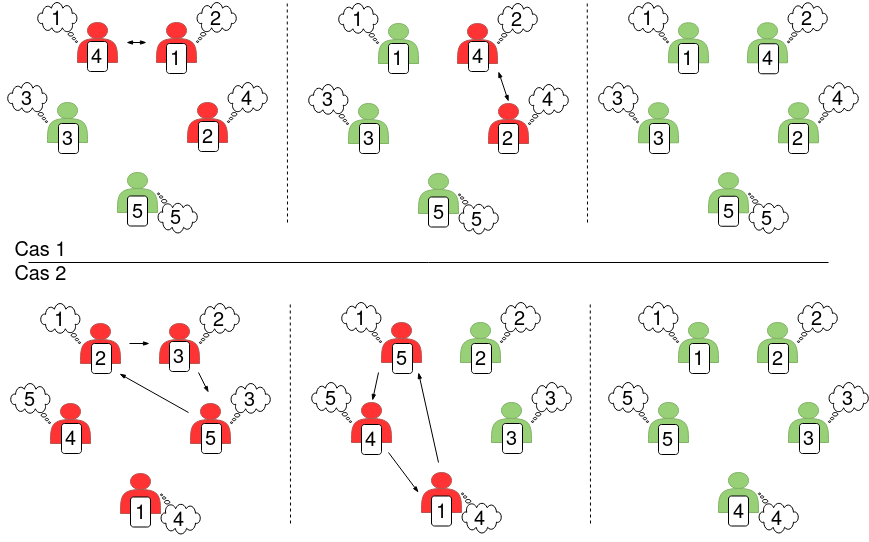
\includegraphics[width=0.9\textwidth]{figures/traders.png}
  \caption{Examples d'échanges à $n=5$ joueurs pour obtenir la distribution désirée. Cas 1, échanges en groupes de 3. Cas 2, échanges en groupes de 3.}
\end{figure}

\subsection{Solution}

\paragraph*{1)}
Toute permutation peut-être décomposée en transposition. 
Un stratégie est d'utiliser un pivot qui sera utilisé pour tous les échanges.

\paragraph*{2)} 
Toute permutation ne peut pas être décomposée en cycles de taille 3. 
En effet, un cycle de taille trois est de signature paire (i.e. décomposable en 2 permutations).
Ainsi, une permutation de signature impaire ne pourra pas être décomposée en une composition de tels cycles.


\section{Une nouvelle librairie en ville}


\subsection{Problème}

Vous êtes le maire d'une ville de 3 habitants, $A$, $B$ et $C$,  vivant sur une droite.
Vous voulez y construire une nouvelle librairie pour faire plaisir à ses habitants.
Chaque habitant sera d'autant plus content que la librairie sera proche de sa maison. 
Vous demandez à chaque habitants de mettre un drapeau sur l'emplacement qu'il préférerait.
La libraire sera construite à l'emplacement moyen des drapeaux (cas 1 de la figure).

\paragraph*{1)} 
L'habitant $C$ connaît les préférences des autres (cas 2 de la figure).
A-t'il intérêt à mentir ? A quel point?

\paragraph*{2)} 
L'habitant $C$ ne connaît pas les préférences données des autres.
Il connaît cependant le résultat d'un sondage effectué auprès de tous les habitants (cas 3 de la figure).
A-t'il intérêt à mentir ? A quel point?

\paragraph*{3)} 
Proposer une nouvelle méthode pour sélectionner l'emplacement de la librairie qui serait moins vulnérable face à quelqu'un comme $C$.

\paragraph*{4)} Généraliser les questions précédentes pour une ville avec plus d'habitants.

\paragraph*{5)} En restant à 3 habitants, pouvez-vous généraliser les question précédentes au cas où les habitants habitent non plus sur une droite, mais dans le plan ? 


\begin{figure}[!h]
  \centering
  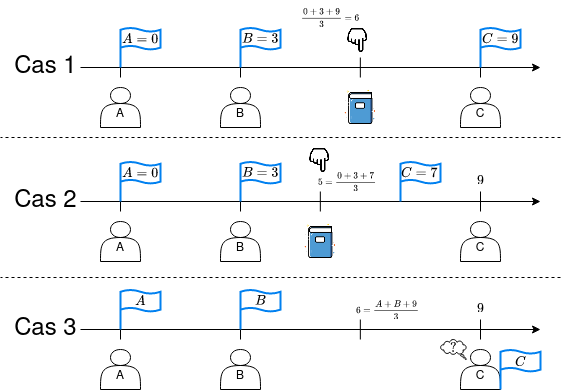
\includegraphics[width=0.50\textwidth]{figures/library.png}
  \caption{
    Cas 1, tout le monde est honnête. 
    Cas 2, l'habitant $C$ ment en connaissant les choix de $A$ et $B$. 
    Cas 3, l'habitant $C$ se demande comment mentir, sachant le résultat du sondage.}
\end{figure}

\subsection{Solution}

\paragraph*{1,2,4)} 
l'habitant $C$ peut mentir et placer la librairie où il le souhaite. Cela reste vrai avec plus d'habitants.

\paragraph*{3)} 
En 1D, une solution moins vulnérable est la médiane des coordonnées. 
Alors, $C$ n'a pas d'intérêt à mentir sur sa vraie préférence. Cela reste vrai avec plus d'habitants.

\paragraph*{5)} 
En 2D pour 3 habitant, une solution moins vulnérable est la médiane géométrique, qui est obtenue en résolvant géométriquement le problème de Fermat \url{https://fr.wikipedia.org/wiki/Probl%C3%A8me_de_Weber}.
Contrairement au cas 1D, ici Jean a quand même un intérêt à mentir.
Cependant il ne pourra pas rapprocher la librairie de chez lui autant qu'il le souhaite.


\section{Le mieux est l'ennemi du bien}

\subsection{Problème}

Vous êtes la mairesse d'une ville de 3 habitants.
Un nouveau fast-food va se construire au centre de la ville, et ça ne vous plaît pas.
La construction est inévitable, seul l'emplacement peut être modifié.
Votre but est de l'éloigner autant que possible de l'emplacement d'origine.

Pour ce faire, vous pouvez proposer un nouvel emplacement à vos habitants, qui sera opposé au précédent lors d'un vote à la majorité.
Chaque habitant votera pour l'emplacement le plus proche de chez lui.

Vous pouvez faire voter un nouvel emplacement autant de fois que vous le souhaiter.
Ce dernier sera alors opposé à celui ayant remporté le vote précédent.


\paragraph*{1)} 
Jusqu'où pouvez vous éloigner le nouveau fast-food ?

\paragraph*{2)} 
Pouvez-vous généraliser à une ville possédant plus d'habitants ?


\begin{figure}[!h]
  \centering
  \includegraphics*[width=0.95\textwidth]{figures/democracy.png}
  \caption{Deux votes successifs. Une nouvelle proposition est en gris. La proposition votée précédemment est en noir.}
\end{figure}


\subsection{Solution}

Le problème est tiré de la vidéo \url{https://www.youtube.com/watch?v=goQ4ii-zBMw} qui illustre les résultats de \cite{MCKELVEY1976472}.

\paragraph*{1)} 
Si les habitants ne sont pas alignés, alors peut importe l'emplacement initial, il est possible de faire des propositions d'emplacement successives de sorte qu'il n'y ai pas de limite à l'éloignement de l'emplacement finalement.
Sans aller jusqu'à le prouver rigoureusement, on peut le constater en se basant simplement sur des constructions géométriques basiques.

\paragraph*{2)}
La réponse et le processus sont les mêmes que pour la question précédente.


\section{Une histoire de boites}

\subsection{Problème}
Vous êtes une équipe de 4 joueurs devant l'entrée d'une pièce, contenant 4 boîtes fermées.
A tour de rôle, vous entrez dans la pièce, ouvrez 2 boîtes et lisez leur contenu.
Vous sortez ensuite de la pièce en la laissant exactement comme elle était à votre arrivée. 
Vous ne pouvez interagir entre vous qu'avant d'entrer dans la pièce.
L'équipe gagne si \textbf{tous les joueurs} trouvent leur propre numéro. 



\paragraph*{1)}
Proposez des stratégies et calculez ou estimez les probabilité de victoire correspondantes.
Vous pourrez tester les performances de vos stratégies en faisant des simulations sur ordinateur.

\paragraph*{2)} Même question avec un plus grand nombre de joueurs. Pour $n$ joueurs, chacun ouvrira $\frac{n}{2}$ boites.

\begin{figure}[!h]
  \centering
  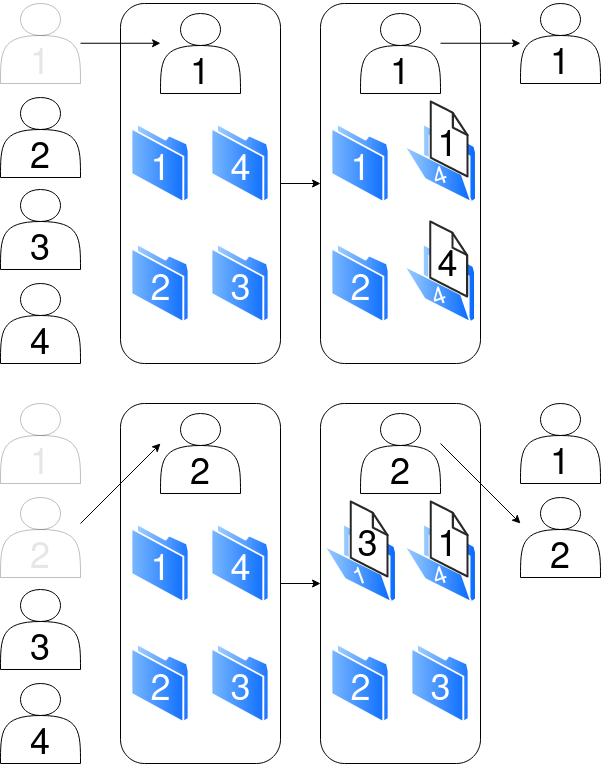
\includegraphics[height=0.3\textheight]{figures/boites.png}
  \caption{Le joueur 1 a trouvé la feuille correspondant à son numéro, il ne fera donc pas perdre l'équipe. Le joueur 2 n'a pas trouvé sa feuille, l'équipe sera donc annoncée perdante à la fin des passages.}
\end{figure}


\subsection{Solution}

Si les $n$ joueurs ouvrent aléatoirement les boites, alors leur chance de victoire est $\frac{1}{2^n}$. 
Construire un arbre de probabilités permet d'obtenir ce résultat.
La stratégie optimale consiste à ouvrir la boite sur laquelle est inscrite son nom, puis celle correspondant au papier de la première, etc. 
Avec cette stratégie, l'équipe de $n$ joueurs à pour probabilité de défaite
\[
  \frac{1}{\frac{n}{2} +1} + \frac{1}{\frac{n}{2} + 2} + \cdots \frac{1}{n} 
  \rightarrow_{n\rightarrow \infty} \ln(2) \simeq 69\%.
\]
Ce résultat s'obtient en dénombrant les permutations de $\{1,\cdots,n\}$ contenant des cycles de taille $k > n/2$.
C'est un problème bien documenté, généralement formulé avec des prisonniers, par example ici \url{https://en.wikipedia.org/wiki/100_prisoners_problem}.

\section{Sauvez le Spyder-verse}

Vous êtes des Spyder-men et Spyder-women de différentes dimensions du Spyder-verse.
Votre mission est d'empêcher le Caïd de mener à bien sont nouveau plan machiavélique.
Pour ce faire, vous devez tous toucher une sphère qui se trouve dans son bureau.

Le problème est que lors de votre infiltration, le Caïd vous a capturé puis enfermé dans différentes cellules, totalement isolées les unes des autres.

A des moments aléatoires, le Caïd choisit l'un d'entre vous et l'amène dans son bureau pour vous interroger.
Ce qu'il ne sait pas 

\newpage
\bibliographystyle{plainnat}  
\bibliography{sujets}

\end{document}